\documentclass[]{politex}
% ========== Opções ==========
% pnumromarab - Numeração de páginas usando algarismos romanos na parte pré-textual e arábicos na parte textual
% abnttoc - Forçar paginação no sumário conforme ABNT (inclui "p." na frente das páginas)
% normalnum - Numeração contínua de figuras e tabelas 
%	(caso contrário, a numeração é reiniciada a cada capítulo)
% draftprint - Ajusta as margens para impressão de rascunhos
%	(reduz a margem interna)
% twosideprint - Ajusta as margens para impressão frente e verso
% capsec - Forçar letras maiúsculas no título das seções
% espacosimples - Documento usando espaçamento simples
% espacoduplo - Documento usando espaçamento duplo
%	(o padrão é usar espaçamento 1.5)
% times - Tenta usar a fonte Times New Roman para o corpo do texto
% noindentfirst - Não indenta o primeiro parágrafo dos capítulos/seções


% ========== Packages ==========
\usepackage[utf8]{inputenc}
\usepackage{amsmath,amsthm,amsfonts,amssymb}
\usepackage{graphicx,cite,enumerate}
\usepackage{makecell}
\graphicspath{ {./images/} }
\usepackage{placeins}
\usepackage{enumitem}


% ========== Language options ==========
\usepackage[brazil]{babel}
%\usepackage[english]{babel}


% ========== ABNT (requer ABNTeX 2) ==========
%	http://www.ctan.org/tex-archive/macros/latex/contrib/abntex2
\usepackage[num]{abntex2cite}

% Forçar o abntex2 a usar [ ] nas referências ao invés de ( )
\citebrackets{[}{]}


% ========== Lorem ipsum ==========
\usepackage{blindtext}



% ========== Opções do documento ==========
% Título
\titulo{SIMIOS - Sistema de Monitoramento Interativo Open-Source de Símios}

% Autor
\autor{Larissa Mangolim Amaral \\%
		Luciana da Costa Marques \\%
		Pedro Orscar Gallo Vaz}

% Para múltiplos autores (TCC)
%\autor{Nome Sobrenome\\%
%		Nome Sobrenome\\%
%		Nome Sobrenome}

% Orientador / Coorientador
\orientador{Professor Livre-Docente Carlos Eduardo Cugnasca}
\coorientador{Professor Doutor Bruno de Carvalho Albertini}

% Tipo de documento
\tcc{Eletricista com ênfase em Computação}
%\dissertacao{Engenharia Elétrica}
%\teseDOC{Engenharia Elétrica}
%\teseLD
%\memorialLD

% Departamento e área de concentração
%\departamento{Nome do departamento}
%\areaConcentracao{Área de concentração}

% Local
\local{São Paulo}

% Ano
\data{2018}




\begin{document}
% ========== Capa e folhas de rosto ==========
\capa
\falsafolhaderosto
\folhaderosto


% ========== Folha de assinaturas (opcional) ==========
%\begin{folhadeaprovacao}
%	\assinatura{Prof.\ X}
%	\assinatura{Prof.\ Y}
%	\assinatura{Prof.\ Z}
%\end{folhadeaprovacao}


% ========== Ficha catalográfica ==========
% Fazer solicitação no site:
%	http://www.poli.usp.br/en/bibliotecas/servicos/catalogacao-na-publicacao.html


% ========== Dedicatória (opcional) ==========
%\dedicatoria{Dedicatória}


% ========== Agradecimentos ==========
\begin{agradecimentos}
Às nossas famílias e amigos, por todo o apoio, suporte e carinho imensuráveis.

Aos professores orientadores, agradecemos a dedicação para o auxílio intelectual e encaminhamento deste trabalho.

À Professora Doutora Cristiane Schilbach Pizzutto, por sua saborosa contribuição para nossa compreensão da óptica do cientista veterinário.

Aos Professores Reginaldo Arakaki, Lúcia Filgueiras e Jorge Kinoshita e ao pós-doutorando Wilian França Costa, pela disposição à orientação e contribuição de conceitos e valores que certamente foram essenciais para o projeto.

Aos demais professores e colegas que contribuíram através de nossa formação como engenheiros e como pessoas.
\end{agradecimentos}

% ========== Epígrafe (opcional) ==========
%\epigrafe{%
%	\emph{``Epígrafe''}
%	\begin{flushright}
%		-{}- Autor
%	\end{flushright}
%}


% ========== Resumo ==========
\begin{resumo}
A execução deste trabalho visa a projeção e implementação de um sistema capaz de auxiliar pesquisadores de saúde e biologia animal no monitoramento comportamental de uma população em estudo. Para tal, foi elaborado um wearable capaz de obter a localização de animais em observação inseridos em ambiente controlado no qual uma rede de sensores é integrada. Tal informação é enviada para uma plataforma onde os dados poderão ser analisados pelo pesquisador remotamente. O desenvolvimento deste sistema tem como finalidade atender às necessidades de monitoramento de símios na reserva natural do Instituto Butantã da Universidade de São Paulo. Contudo, pretende-se que sua aplicação seja possível em distintas reservas, para a observação de diferentes animais e que possa eventualmente ser expandido para captar demais variáveis de controle relevantes para o biólogo. Finalmente, o sistema obtido cumpre os requisitos definidos e demonstra escalabilidade.

\textbf{Palavras-Chave} -- Monitoramento animal remoto, Redes de sensores sem fio, Embarcado.
\end{resumo}

% ========== Abstract ==========
\begin{abstract}
This study presents the design and implementation of an entire system capable of assisting animal health and biology researchers monitoring the object of study. Therefore, an embedded wearable was programmed so that the system could provide the researcher remotely with the observed animals’ location. For that to happen, they would have to be living in a natural reserve mapped by a wireless sensor network. This system’s purpose is to meet Instituto Butantã’s needs regarding monitoring simios inside the reserve. However, it is expected that this system is also applicable inside many different reserves, for distinct mammals observation and open to be expanded so that it shall be able to monitor as many other control variables the biologist finds relevant. The final work meets the defined requirements and shows scalability.

\textbf{Keywords} -- Remote animal monitoring, Wireless sensor network, Embedded.
\end{abstract}

% ========== Listas (opcional) ==========
\listadefiguras
\listadetabelas

% ========== Listas definidas pelo usuário (opcional) ==========
\begin{pretextualsection}{Lista de abreviaturas e siglas}

GPS \textit{Global Positioning System}

BLE \textit{Bluetooth Low Energy}

MVC \textit{Model-view-controller}

GAP \textit{Generic Access Profile}

GATT \textit{Generic Attribute Profile}

RFID \textit{Radio-Frequency Identification}

RSSI \textit{Received Signal Strength Indication}

\end{pretextualsection}

% ========== Sumário ==========
\sumario



% ========== Elementos textuais ==========

%\chapter{Introdução}
	
\section{Objetivo}
Este trabalho visa o projeto e implementação de um sistema capaz de obter a posição relativa de macacos em reservas, dentre outros dados do ambiente ou do animal.

A composição do sistema prevê (1) dispositivos embarcados inseridos em mochilinhas anexadas ao macaco, que, em conjunto, compõem (2) uma rede de sensores para adquirir as informações necessárias do ambiente e enviá-las para (3) um servidor. Este realiza o processamento e armazenamento dos dados que serão injetados em (4) uma interface em software disponível para o usuário.

A discriminação do sistema é melhor realizada nos capítulos 4 e 6.



%\chapter{Aspectos Conceituais}
Alguns dos principais conceitos para compreensão e contextualização deste projeto são trabalhados neste capítulo.
	
\section{Macacos e Reservas Naturais}
Para melhor compreensão do aspecto biológico que este trabalho toca, foi realizada uma entrevista com a professora Cristiane Pizzutto, que pode ser vista na íntegra no apêndice 1 deste documento.

A partir desta, foi possível quantificar alguns parâmetros importantes para o dimensionamento do projeto, tal como a quantidade comumente observada de animais em bandos de reservas e cativeiros, para qual foi assegurado que, considerando um bando de dez macacos, estaríamos abrangendo seguramente o suficiente.

Também foi possível notar como a tarefa de observação para aquisição de dados relativos aos animais, tais como sinais vitais, movimentação e alimentação, é exaustiva, toma tempo e pode ser objetiva o bastante para que possa ser realizada por um sistema remoto.

A parte subjetiva do levantamento de dados está relacionada às atividades e interações dos animais, que normalmente só podem ser adquiridos por observação direta. Essa é a parte que nosso projeto tenta abordar e que nos fez perceber que talvez, para cativeiro, o auxílio de câmeras com alguma inteligência seria bem vindo.

Outra questão levantada é de como estes dados são digeridos. A pesquisadora aponta que a manipulação dos dados é manual e que utilizam planilhas para obter estatísticas. Considerando a quantidade massiva de dados, seria interessante pensar em injetar conceitos de Big Data.

\section{Tecnologias Potenciais}
\textbf{Redes de Sensores Sem Fio}

A emergência da tecnologia de Redes de Sensores Sem Fio (RSSF) permitiu não somente o monitoramento das variáveis de um objeto, mas também o supervisionamento de todo o contexto em que ele está incluído e da interação dele com os demais pontos do sistema sendo sensoriados.

RSSFs são especialmente relevantes quando se tratando de ambientes cuja área que deve ser coberta é muito extensa. Estas redes são compostas por nós interligados, em que cada nó deve ter sensores, processamento, memória, antena e bateria independentes e sustentáveis.

Dada essa composição, as RSSFs são capazes de satisfazer áreas de cobertura muito extensas e são ótimas para criar integração entre elementos que estão, localmente, constantemente conjuntos.

Por isso, compõem uma tecnologia ótima para organizações biológicas, que envolvem grandes populações distribuídas, sendo, portanto, frequentemente aplicadas em sistemas agrícolas.

Como enfatizado por Handcock (2009), para animais essa utilidade também é incluída, mas prevê algumas ressalvas. Uma delas considera a situação de que o animal de vida livre pode permanecer por semanas fora do alcance de pontos de acesso que recebam seus dados e, por esse motivo, cada nó da rede deverá possuir bateria e memória suficientemente robustas. Para reduzir o tempo de ausência de resposta de um determinado indivíduo, é possível implementar escuta nos próprios nós da rede, de forma que os animais que entrarem em contato entre si mantenham as informações dos demais, aumentando a chance de que algum deles possa transmiti-las para o servidor no alcance de pontos de acesso. Essa prática, no entanto, exige ainda mais energia e armazenamento.

RSSFs são, por vezes, estudadas para posicionamento em ambientes internos, principalmente atreladas ao uso de pontos de acesso Wi-fi, que já são naturalmente alocados nesses espaços para uso de internet.

\textbf{Rádio}
A aplicação tecnológica para rastreamento de animais mostra-se insistente no uso de transmissores de rádio por muitos anos, por mais que a tecnologia de localização para aplicações humanas já o tenha superado de longe.

O RFID foi bastante usado para obter informações relacionadas à condição do animal identificado. Recentemente, estes transmissores têm sido também utilizados para detectar encontros sociais entre animais através de picos de intensidade do sinal de rádio sendo transmitido.

\textbf{GPS}
A emancipação do GPS aplicado ao smartphone praticamente trivializou a tarefa de localização, principalmente quando associada à mobilidade e roteamento.

A integração de tal tecnologia em sistemas biológicos demonstra uma tentativa de integrar o sensoriamento da interação do animal com o ambiente, como é salientado por Handcock [5].

O GPS, no entanto, tem uma série de complicações. Primeiramente, sua precisão em baixa escala é bem complicada. Handcock afirma que para obter boa acurácia, é necessário ter uma taxa de amostragem relativamente alta, o que é bastante ruim para a sustentabilidade da memória e da energia do sistema.

Um outro problema está relacionado à pouca praticidade do módulo GPS, que apresenta peso relativamente elevado (aproximadamente 10g) dependendo do animal que está sendo rastreado.

\section{Modelos Comerciais}
Alguns modelos de coleiras voltadas a mamíferos são citadas na tabela a seguir. Os produtos são fornecidos pela empresa ATS que, infelizmente, não discrimina o porte recomendado do animal usuário em seu site, portanto só foi possível inferir o peso que o dispositivo deste projeto deveria ter confirmando o que havia sido relatado pelos pesquisadores: de algo de no máximo 10g, uma vez que macacos menores pesam cerca de 400g.

Por outro lado, foi possível conceber alguns potenciais modelos para o invólucro do produto final deste projeto, principalmente no que diz respeito ao material utilizado.

\begin{table}[ht]
\centering
\caption{Exemplos comerciais de coleiras de rastreamento de mamíferos da ATS}
\vspace{0.5cm}
\begin{tabular}{l|ccc}
\hline
Nome & \makecell{SM17X0 Mammal \\ Collar, X-Small} & \makecell{M15X5 Mammal \\ Zip-Tie Collar} & \makecell{W500 Wildlink GPS \\ Logger, Small Collar} \\
Imagem & 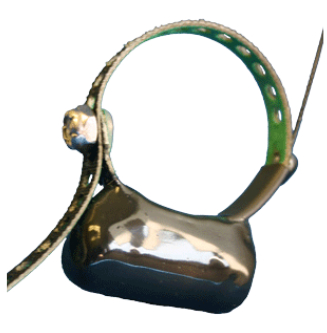
\includegraphics[scale=0.5]{ATS1} & 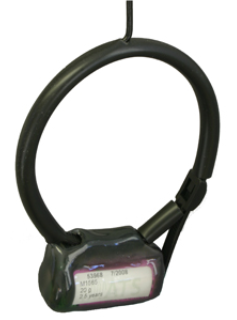
\includegraphics[scale=0.5]{ATS2} & 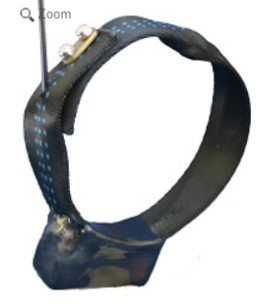
\includegraphics[scale=0.5]{ATS3} \vspace{0.4cm}\\

Peso & 9 a 16g & 10 a 40g & 65 a 115g \vspace{0.4cm}\\

Bateria & Lítio / 156 a 282 dias & Lítio / 195 a 596 dias & AA / 1,75 a 3,5 anos \vspace{0.4cm} \\

Material & 
\makecell{- Coleira de \\ \textbf{neoprene} \\
- Encapsulamento \\ de resina a prova \\ de água} &
\makecell{ - Coleira de \textbf{tubo} \\ \textbf{de plástico (cable-tie)} \\
- Encapsulamento \\ de resina a prova \\ de água} &
\makecell{- Coleira de \textbf{neoprene} \\ \textbf{ou nylon} }   
\end{tabular}
\end{table}

Como visto no item anterior, comercialmente é utilizado rádio na maior parte dos casos (M17X0 e M15X5) e, eventualmente, GPS (W500 - para o qual é possível notar que exige um peso bem superior ao limite estabelecido de cerca de 10g).
\FloatBarrier

\section{Algoritmos}
Inicialmente, é necessário compreender uma forma de calcular a posição dos animais através da distância entre macaco e ponto de acesso. De praxe, em RSSFs este cálculo pode ser feito de duas formas.

A primeira delas é utilizando a intensidade do sinal (\textit{Received Signal Strength Indication} - RSSI). O cálculo da distância, neste caso, é dado pelo seguinte modelo proposto pela Texas Instruments, que é melhor detalhado por Dong e Dargie (2012).

\begin{equation}
RSSI = -10 \times n \times \log_{10} d + A
\end{equation}

Sendo:
\begin{itemize}
\item d a distância em metros
\item RSSI a intensidade do sinal em dBm
\item n a constante de propagação do sinal
\item A a intensidade do sinal para 1 metro de distância
\end{itemize}

Essa é uma maneira simples de baixo custo de implementação, porém, como é bem destacado por Larsson (2015), dada a alta variação de n devido a suscetibilidade do sinal à interferência do meio, demonstra-se um tanto imprecisa.

A constante de propagação pode ser determinada empiricamente. Se sabe n=2 para o vácuo; no ar, valores coerentes estão entre 2.7 e 4. A determinação da constante para este projeto pode ser observada no apêndice.

Outra forma seria calcular a distância sabendo a velocidade de propagação do sinal no meio, dado o tempo que demora para que o sinal seja recebido a partir da implementação de um eco. Idealmente esta é uma abordagem muito mais precisa, que só é impossibilitada em casos que o hardware utilizado não possua relógio. No entanto, qualquer deficiência na temporização e sincronização, por menor que seja, pode comprometer a precisão de tal metodologia.

Para este projeto, pretende-se implementar a primeira forma e verificar a precisão da mesma.

Além disso, foi requerido desenvolver um algoritmo para obtenção do mapeamento da posição dos macacos. Este tema já havia sido discutido por Amaral e Biscaro (2017) e, para este caso, o único algoritmo que se fez praticável é a trilateração.

\begin{figure}[ht]
  \centering
    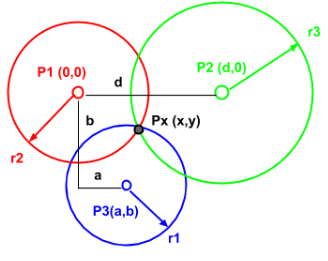
\includegraphics[scale=1]{trilateracao}
  \caption{Algoritmo de trilateração (Fonte: autores)}
\end{figure}
\FloatBarrier

Dada a figura acima, o ponto P pode ser calculado conhecendo-se os pontos fixos P1, P2, P3, as distâncias entre eles e as distâncias entre os mesmos e P (r1, r2 e r3, respectivamente). Assim, é criado um sistema compondo as três equações de circunferências, resultando no seguinte equacionamento.

Se x1 $\neq$ x2:

\quad $\alpha = \dfrac{x1 - x3}{x2 - x1}$

\quad $\beta = 2 \times [(y3 - y1) + \alpha(y2 - y1)]$

\quad Se $\beta \neq$ 0:

\quad \quad y = $\dfrac{(x3^2 - x1^2) + (y3^2 - y1^2) + (r1^2 - r3^2) + \alpha[(x2^2 - x1^2) + (y2^2 - y1^2) + (r1^2 - r2^2)]}{\beta}$

\quad \quad x = $\dfrac{2y(y1 - y2) + (x2^2 - x1^2) + (y2^2 - y1^2) + (r1^2 - r2^2)}{2(x2 - x1)}$

Senão, se x2 $\neq$ x3:

\quad $\alpha = \dfrac{x1 - x3}{x3 - x2}$

\quad $\beta = 2 \times [(y3 - y1) + \alpha(y2 - y3)]$

\quad Se $\beta \neq$ 0:

\quad \quad y = $\dfrac{(x3^2 - x1^2) + (y3^2 - y1^2) + (r1^2 - r3^2) + \alpha[(x3^2 - x2^2) + (y3^2 - y2^2) + (r2^2 - r3^2)]}{\beta}$

\quad \quad x = $\dfrac{2y(y2 - y3) + (x3^2 - x2^2) + (y3^2 - y2^2) + (r2^2 - r3^2)}{2(x3 - x2)}$

Se não couberem nenhum desses dois casos, sabemos que as circunferências não possuem ponto de intersecção,

%\chapter{Metodologia do Trabalho}
Seguindo as orientações de projeto de embarcados indicadas pelo professor orientador (Cugnasca, 2018), inicialmente é necessário levantar e descrever os requisitos funcionais e não funcionais do sistema - o que é feito já no capítulo seguinte.

A segunda etapa consiste na definição da arquitetura do projeto, para qual os possíveis componentes são associados estabelecendo uma composição que cubra os requisitos funcionais do projeto. A arquitetura é descrita no capítulo 6.

A seguir, aos componentes visíveis no plano físico, o que é feito no capítulo 5. Por fim, é implementado a arquitetura que foi projetada.

É adotada metodologia top-down visto que primeiro é definido o produto que se deseja obter para poder segmentar as tarefas a serem realizadas em micro serviços.

Ao mesmo tempo o projeto utiliza duas abordagens. Em alguns aspectos é utilizado o modelo em cascata, pois, por se tratar de um trabalho de formatura, é natural que algumas otimizações sejam reservadas para projetos futuros. Por esse ponto de vista, é como se cada projeto fosse uma curva na espiral.

Por outro lado, dada a abrangência tecnológica do projeto, em frentes como a interface será adotado o modelo espiral, pois neste caso modificações eventuais são menos custosas em tempo e orçamento. Portanto, estão planejados testes de usabilidade do software em diversas etapas de produção.


%\chapter{Especificação de Requisitos de Sistema}
O funcionamento essencial do sistema, o que define seus requisitos funcionais, requer que a posição dos macacos seja possível de ser medida, armazenada e mostrada para o usuário.

Além desses, são levantados os requisitos não funcionais, que trabalham aspectos necessários e complementares para o bom funcionamento do sistema, muitas vezes previstos pelo público solicitante do mesmo.

No SIMIOS, os principais requisitos não funcionais foram apontados por pesquisadores biólogos e veterinários com experiência em monitoramento de macacos. Dentre eles, está que o peso da mochila que será anexada ao animal não deveria ultrapassar 10g para não influenciar em seu comportamento nem sobrecarregá-lo, visto que o principal grupo de foco (saguis) tem peso médio de 400g. Para isso, é interessante que todos os componentes da mochila sejam o mais leves possível.

Outra situação apontada é o fato de que toda vez que a bateria do aparelho tiver de ser trocada, o veterinário deverá capturar o macaco e sedá-lo, o que é bastante prejudicial para a confiança que o animal constrói pelo ser humano. Dessa forma, é desejável que a eficiência energética do dispositivo embarcado seja alta para que a bateria tenha de ser trocada com a menor frequência possível.

Além da mochila do animal, espera-se que os dados coletados sejam confiáveis. Isso envolve garantir a autenticidade e a ausência de erros, ou seja, que eles estejam sendo de fato enviados íntegros pelo macaco a quem estão associados. Assim, evita-se casos em que o dispositivo possa ter sido removido acidentalmente e, por exemplo, enroscado em uma árvore ou em que existam interferências ruidosas no sinal capazes de alterar significativamente as medições enviadas. Também é relevante que o acesso à informação seja possível somente para pessoas autorizadas, envolvendo conceitos como autenticação e codificação.

SIMIOS é um sistema que, estruturalmente, poderia ser contextualizado em praticamente qualquer aplicação que se tenha algo a ser rastreado, seja um ser vivo ou não, para qual a precisão do GPS seja insuficiente. Portanto, de maneira geral, também é interessante que o sistema tenha escalabilidade em todos os aspectos - que os dispositivos embarcados nos animais possuam sensores diversos e que, possivelmente, toda a aplicação suporte que uma quantidade maior de variáveis e de usuários seja inserida.

Por fim, é sempre relevante que a interface com o usuário siga princípios de UX, especialmente se considerando que uma quantidade grande de dados deve ser visualizada de forma intuitiva e simples pelo pesquisador.

\begin{figure}[ht]
  \centering
    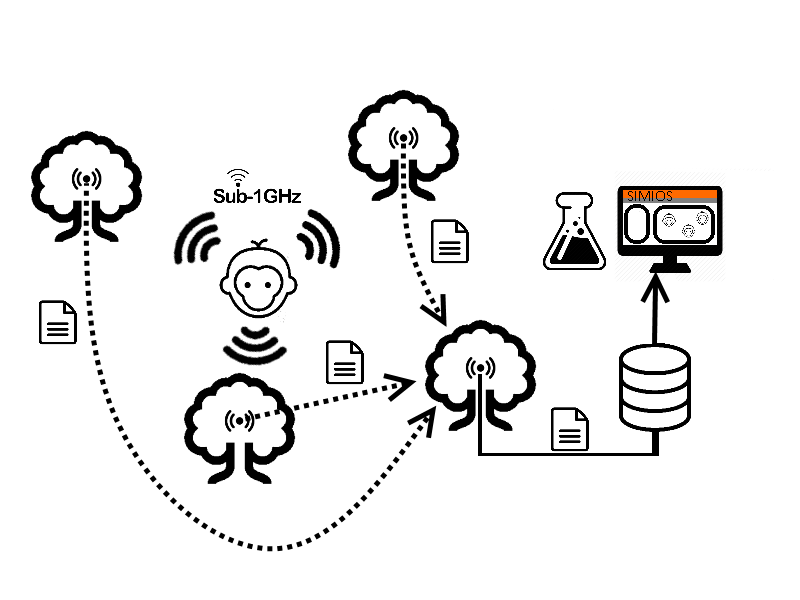
\includegraphics[scale=0.7]{esquematico}
  \caption{Resumo gráfico do sistema (Fonte: autores)}
\end{figure}
\FloatBarrier

%\chapter{Tecnologias Utilizadas}
Considerando os aspectos discutidos no capítulo 2 sobre possíveis e impossíveis instrumentos para o nosso contexto, por fim foram selecionadas as tecnologias que serão efetivamente utilizados no projeto, as quais são descritas neste capítulo.

\section{Dispositivo Embarcado}
Partindo disso, selecionou-se a plataforma de desenvolvimento do Sensor Tag da Texas Instruments como componente embarcado de cada macaco. Trata-se de uma placa leve que contém 6 sensores, incluindo de temperatura, e comunicador BLE. Seu datasheet pode ser encontrado nas referências deste trabalho.

\begin{figure}[ht]
  \centering
    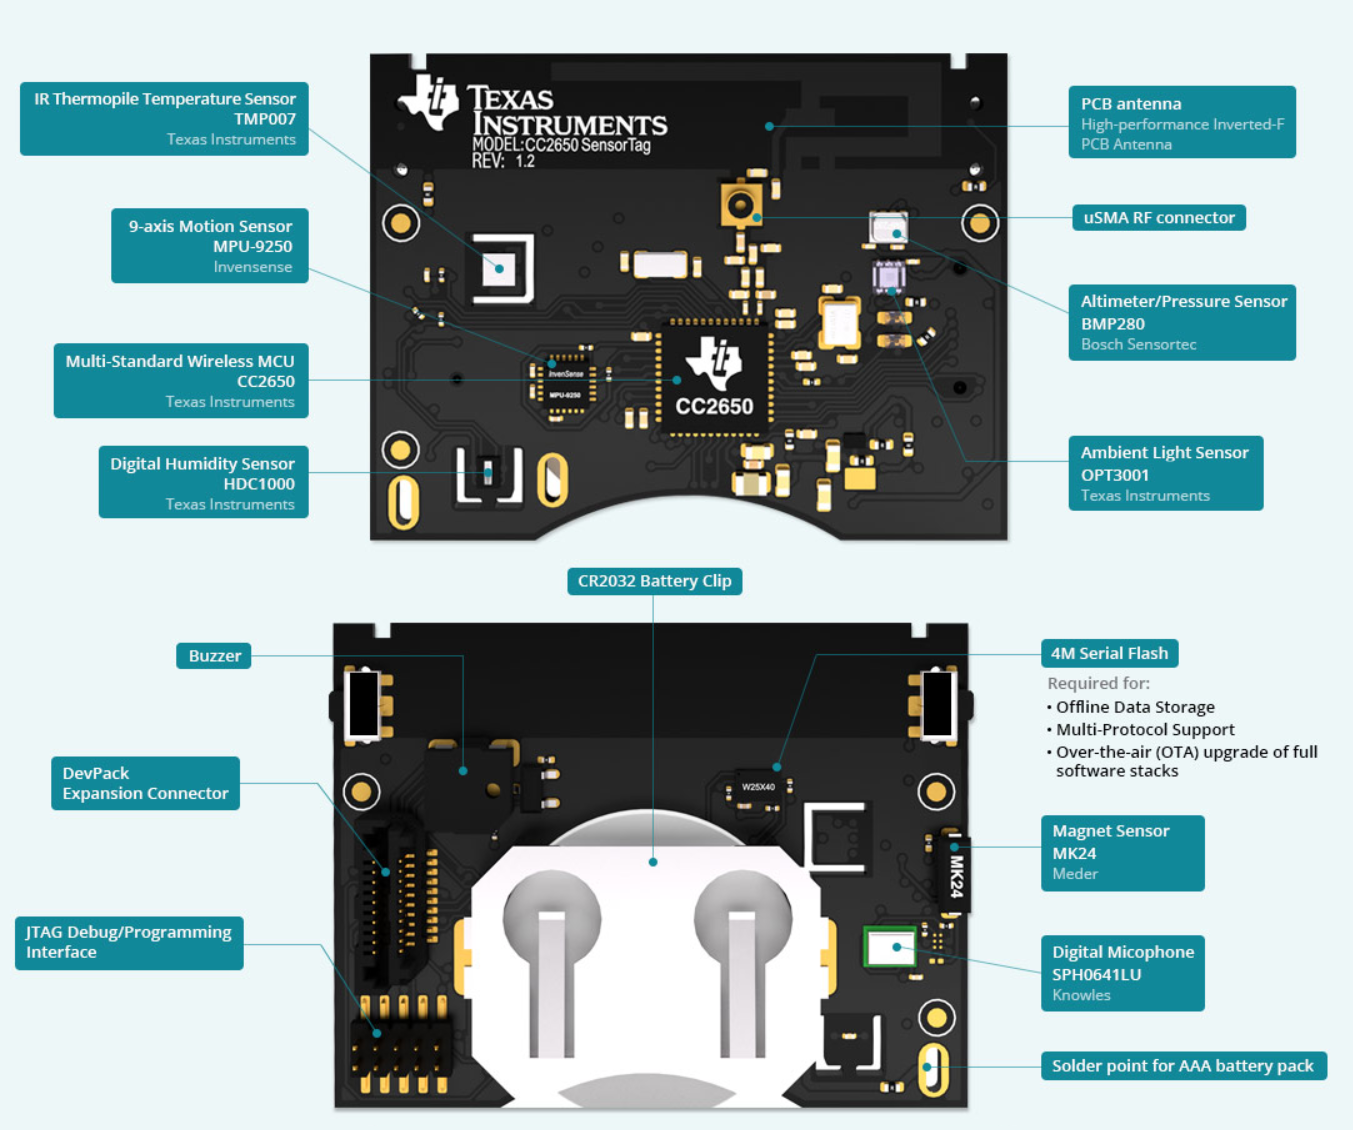
\includegraphics[scale=0.5]{sensortag}
  \caption{Componentes do Sensor Tag (Fonte: extraído do site da Texas Instruments)}
\end{figure}

Foi utilizado um Raspberry Pi 2 para receber por BLE os dados de cada Sensor Tag e enviá-los por Wi-fi para o servidor, que pode ser local ou em nuvem. 

\section{Servidor}
Foi escolhido o banco de dados relacional MySQL da Oracle por se tratar de um sistema open source simples, embora completo.

O projeto SIMIOS prevê o rastreio de animais em reservas, o que envolve, como visto anteriormente, no máximo cerca de 50 animais em grandes reservas. Dessa forma, sabemos que não envolve sobrecarga de acessos por segundo e mesmo isto poderia ser corrigido com buffering.

Um ponto negativo do MySQL é que sua escalabilidade pode ser prejudicada - cada servidor tem um tamanho limitado e cada set de dados só pode ser alocado em um servidor (não suporta particionamento), o que pode ser prejudicial em casos que deseja-se guardar no banco grande quantidade de dados. Para corrigir tal empecilho é possível implementar importação de dados.

\section{Software}
Para desenvolvimento do programa computacional que é executado no servidor, foi escolhida a linguagem de programação Java, com suporte de frameworks Spring e JPA, facilitando principalmente os processos de queries do banco de dados, de autenticação e autorização e de mapeamento de interface model-view-controller (MVC).

Por se tratar de uma aplicação de histórico de dados, pouquíssimo processamento está previsto e a computação pode ser realizada em tempo real pelo computador do usuário. Dessa forma, não se faz necessário o uso de linguagem de programação de execução eficiente (C++, por exemplo).


\include{projeto-implementacao}

\include{testes-avaliacao}

\include{consideracoes-finais}

% ========== Referências ==========
% --- IEEE ---
%	http://www.ctan.org/tex-archive/macros/latex/contrib/IEEEtran
\bibliographystyle{IEEEbib}

% --- ABNT (requer ABNTeX 2) ---
%	http://www.ctan.org/tex-archive/macros/latex/contrib/abntex2
%\bibliographystyle{abntex2-num}

\bibliography{}


% ========== Apêndices (opcional) ==========
\apendice
\chapter{Entrevista com a profª Drª Cristiane Schilbach Pizzutto}

Para agregar ao conhecimento interdisciplinar necessário para a projeção deste trabalho, foi realizada entrevista com a professora Cristiane Pizzutto, da Faculdade de Medicina Veterinária da USP, cuja redação foi documentada a seguir com o consentimento da doutora.

\textbf{09 maio 2018 - São Paulo, SP}

P: Quantos anos você tem?

R: Quarenta e cinco.

P: Qual a sua área de atuação?

R: Eu trabalho com a  parte de animais silvestres em cativeiro. Mais especificamente, eu trabalho com enriquecimento orientado: avalio o estresse desses animais, mas também todo um monitoramento comportamental e endócrino deles em função dos ambientes que eles vivem e também o recurso de animais silvestres, muito voltado para a conservação. Hoje o cativeiro tem um papel importante na conservação desses animais, por isso muitas espécies a gente tem que estar preocupado em reproduzir para depois tentar reintroduzir no meio ambiente.

P: Quanto aos animais, essa monitoração é feita em laboratórios?

R: No laboratório a gente só faz a parte de dosagens hormonais dos animais.


P: Como se chama o lugar dos animais?

R: Cativeiro, zoológicos, aquários. Nesses espaços, a gente fala que é o recinto desses animais. O cativeiro nada mais é do que a privação da liberdade desses animais, não podem fugir, o que não está em vida livre está cativo. Eu trabalho com estes animais.


P: Quantos animais você acha que acaba monitorando? Tem o controle de animais que controla ao longo do tempo ou você vai ao local e tem alguns animais e você conhece eles na hora?

R: Então, eu não trabalho com animais de vida livre, é diferente de uma pesquisa de quem trabalha em campo e quem trabalha com animais de cativeiro. No meu caso, eu conheço os animais e todos estão envolvidos no projeto que eu trabalho. Meu acompanhamento é quase individual. Eu tenho como saber o que acontece com ele do ponto de vista comportamental e hormonal.


P: Quantos animais são monitorados em um projeto?

R: Depende. Quando se trabalha com animal silvestre, a gente trabalha com um N reduzido, mas geralmente é aquela quantidade daquele cativeiro. Por exemplo, com aves geralmente a gente trabalha com mais animais: num projeto com araras temos mais do que 25 araras, mas quando trabalhamos com espécies mais raras, como a onça pintada, temos só uma ou duas em cativeiro. Quase nunca passa de trinta, nosso número mais comum é 1, o que dificulta fazer estatísticas e com uns 7 já estamos dando pulos de alegria.


[Estamos pensando em 10 saguis.
Maravilhoso.]


P: Quanto tempo você dedica às tarefas de ir até os animais? Quanto tempo demora isso?

R: Depende. No meu trabalho, quando a gente mexe com a parte comportamental. Em qualquer trabalho com comportamento, exige ao menos vinte a trinta horas de observação, que eu tenho que dividir ao longo de um período para obter uma estatística sensata. Além disso, tenho que determinar qual período do dia eu posso observar esses animais, por que têm momentos do dia que eles estão mais ativos e momentos que eles estão menos. Porque eu quero a maior quantidade de informações comportamentais pra mim dos períodos mais ativos. Isso também é diluído ao longo da metodologia dos trabalhos. Como eu trabalho com mudanças ambientais, eu faço sempre o antes e o depois: Eu faço de trinta a quarenta horas antes e de trinta a quarenta horas depois. Por isso eu tenho que dar uma boa lapidada neles que eles vão ter que ter paciência e tempo, porque demanda concentração nesses trabalhos. Quando eu faço coleta de material para análise hormonal é coisa rápida, às vezes trabalho com fezes que nem coloco a mão no animal; é um método novo que é pouco invasivo. Mas se for trabalhar com sangue tem que dar anestesia.


P: Essas trinta a quarenta horas são de observação direta?

R: Direta, tem que estar na frente do animal e fazer registros. A gente faz o que se chama de histogramas, que são formas de análise do comportamento. Tem vários métodos: posso observar o animals de forma instantânea, de tempos em tempos eu faço o registro; ou posso fazer um registro contínuo onde eu observo o dia inteiro sem pausa. Tem várias formas. Eu acho que o sistema de vocês o mais interessante é o envio de informações instantâneas. 


P: Essa é minha outra pergunta, você acha que as informações que você acaba indo a campo monitorar dos animais, se você acha que essas informações podem ser captadas e enviadas para laboratório? Se isso ajuda?

R: Não sei se vocês conseguem esse tipo de informações, porque não sei se sua placa consegue mandar a informação de que o animal tá comendo, o que eu posso ver quando tô observando o animal. Isso me interessa porque cativeiros geralmente tem o histórico de ser muito ruins, eles não atendem às necessidades dos animais. Por exemplos alguns primatas comem no chão, outros vivem em extratos de 10 metros, outros de 15 metros. Com a observações em cativeiro, eu consigo fazer essa avaliação, olha eu vejo um animal que se alimenta na faixa de 2-3 metros, vocês podem não conseguir fazer essas observações e essas são informações valiosas pra mim. Não sei se vocês vão conseguir ter acesso a essas informações e enviá-las pro laboratório.


P: Para esse tipo de coisa, você acha válido ter câmeras?

R: Sim.


P: Vocês têm câmeras em alguns cativeiros já?

R: Instaladas, sim, mas elas são fixas e eles filmam os animais. Mas vocês com esse sistema, o ideal seria você ter uma câmera para enxergar o que o animal tá fazendo.


P: Quais são procedimentos padrões, tem alguma rotina fixa para esse tipo de pesquisa ou depende do animal ou do cativeiro?

R: Depende de várias coisas: da instituição, que tem que liberar o acesso pra gente poder observar os animais; e como o projeto começa, a gente tem que seguir a metodologia. Vamos supor que eu tenha 6 meses pra fazer a linha de base que é fazer as observações primárias para descobrir qual momento do dia o animal tá mais ativo e a gente divide o número de horas durante 6 meses, cada dia que você for lá você vai observar 1 hora nesse período de maior atividade porque nesses 6 meses tem que fazer as quarenta horas de registro.


P: A avaliação inicial do período de atividade é feita por observação direta também?

R: Sim, mas é diferente de como a gente observa. Por exemplo, se eu tenho 5 animais num ambiente, a cada 5 minutos durante um dia inteiro, por 3 dias, ela vai observar e falar que eu tenho 2 animais ativos às 7:00 e 3 inativos, ai ela vai fazendo os registro de 15 em 15 min para fazer um gráfico de atividade e inatividade, e a gente consegue ver qual momento do dia a gente tem mais e menos animais ativos. Ativo ele ta fazendo qualquer coisa, inativo é que ele ta deitado sem fazer absolutamente nada, porque, primatas em especial, são animais que têm variabilidade comportamental, eles fazem absolutamente tudo ao mesmo tempo, quando a gente vai fazer registro a gente fica louca de tanta informações que eles passam pra nós.


P: Esse dados... tem uma formatação dos dados, vocês usam algum tipo de programa?

R: A gente já tentou usar um que o nome eu não lembro… mas parece um aparelho que registra água e luz. Mas eu não consegui me adaptar com ele, porque ele me fala assim: agora tá na hora de registrar, mas às vezes o animal tá representando um comportamento que não tá cadastrado no sistema e o sistema não aceita. Prefiro fazer tudo no papel e os alunos no final do dia contabilizam os comportamentos e jogam em uma planilha do excel, porque esse aparelho tem que ser pré programado para todos os comportamentos que o animal pode ter e nem sempre o animal executa o comportamento.

Seria melhor alguma coisa mais aberta ou personalizada. Seria fantástico.
A gente trabalha com sigla, porque tem que ser muito rápido, tipo, comendo depois a gente sabe que é CO.


P: Como é feito para localizar o animal dentro de cativeiro? Como é feito para identificar o animal?

R: Muitos a gente consegue saber quem é quem, principalmente por características externas, às vezes tem um defeito na orelha ou uma pelagem diferente e primata tem uma feição muito diferente entre eles, é fácil.

Mas por exemplo, em um trabalho que estou orientando no aquário de São Paulo com cangurus, e aí é uma coisa difícil de identificar e a gente vai pro coletivo e não pro indivíduo. A gente registra pelo grupo e fazemos um método chamado de scan. Os registros podem ser contínuos ou instantâneos, por intervalo de tempo, mas nesses caso eu preciso fazer um scan do grupo e instantâneo, já que contínuo é impossível, fazendo um registro do que cada animal está fazendo sem identificar quem é quem.


P: No contínuo você faz um log a todo momento de todas as atividades independente do tempo?

R: Eu uso o contínuo quando eu quero fazer um registro detalhado de como o animal come, ai eu olho o animal: pegou a comida, levou até a boca, devolveu, engoliu, o registro de como ele come. No meu caso é mais interessante fazer o instantâneo, porque eu foco no tipo de comportamento e acabo tendo milhares de registros no final de um dia, imagina no final de um projeto. Eu cheguei a ter 170.000 em uma planilha de excel com um gorila que eu trabalhei durante 8 anos e aí eu consigo ter frequência de ocorrências. Eu trabalho com quantidade de comportamento, eu transformo um em milhares de dados (informações).

Fica coisa pra caramba, aí eu dou uma driblada na estatística, por que 1 não é estatística, mas com 170.000 já dá pra fazer estatística. A gente faz o que a gente pode com animais tão ameaçados. Não tem, não adianta querer ter. Isso é difícil de convencer a comunidade científica, nem todo mundo é da área e as pessoas não entendem a importância de trabalhar com um indivíduo. Não adianta querer ter pelo menos 2, não tem.


P: Voltando, sobre o programa que você falou que trabalhava com anotação no papel, tem algum outro instrumento que você usa?

R: Uso muito uma câmera fotográfica para filmar porque o comportamento é dinâmico. Nem sempre as pessoas entendem quando a gente descreve e fazer registro é muito importante. E às vezes binóculo, só para enxergar melhor os comportamentos. Para registro: foto filmagem e papel. Basicamente isso.


P: Os animais se comportam muito diferente quando você observa eles?

R: Sim, muitos se estressam com a presença de humanos, por isso a gente faz uma etapa de socialização, então a gente fica um dia por perto pra ele ver a gente e se acostumar. Quando ele se acostuma com a gente lá e faz as observações. O que eles têm é muito problema de comportamento pro cativeiro que eles tão, aí em cativeiro é muito ruim e não atende as atividades deles do dia a dia e eles têm comportamentos anormais, estereotipados. Aí tem um monte de coisa, é com isso que eu trabalho. Aí eu entro com a técnica de enriquecimento ambiental que é pra restaurar os comportamentos normais que eles tem e melhorar a qualidade de vida deles e quando isso acontece, a gente tem sucesso na reprodução. Esse é o segredo de manter zoológico hoje, não é pra manter só por manter, a gente tem que dar qualidade de vida pra eles pra que eles justifiquem o animal estar preso.


P: Seu maior interesse é aproximar o comportamento que eles têm em cativeiro pro que eles têm fora?

R: Isso, quero resgatar comportamentos que eles perdem. Eles perdem certos comportamentos em cativeiro: eles tem tanto estresse que acabam tendo mais comportamento anormais do que naturais e típicos da espécie e o objetivo é resgatar esses comportamentos naturais.


P: Eles não ficam todos em reservas?

R: Não temos reservas para todos. Eu vou falar pra vocês, é triste isso, mas temos ativistas que falam que temos que abrir portas do zoológico e soltar. Eles vão morrer se a gente soltar. Não tem cadeia alimentar que suporte esses animais: os ambientes tão destruídos. Se a gente fizer uma soltura em massa, a gente não vai ter suporte alimentar para todos. A gente vai matá-los com certeza. Não tem o que fazer.  

A questão é essa: tem que considerar a situação que o animal tá vivendo e que o ambiente natural tá vivendo. Há 10 anos, eu não defendia tanto cativeiro quanto eu defendo hoje. Agora eu preciso defender a existência de cativeiro, porque nós vamos perder os últimos membros das espécies. Trabalhar pela preservação do que nós temos em prol da conservação da natureza.


P: Esse processo de socialização com os animais em cativeiro, como ele é feito? Leva muito tempo para eles se acostumarem? 

R: Eu comecei com um trabalho com um gorila que tinha no zoológico de São Paulo, que era solitário por muitos anos. Quando eu voltei desse estágio nos EUA, que eu vi que eles faziam essa questão de enriquecimento ambiental e tudo, que aqui no Brasil não tinha, e foi inédito. Eu comecei observando ele a distância. Só observar, até uma hora que eu percebi que o animal me observava, não mais eu observava ele, ai eu peguei e sentei na frente da grade dele e fique fazendo uma aproximação porque eu queria condicioná-lo. Esse processo demorou 6 meses. Porque era um gorila, um exemplar raro; que você não pode olhar no olhos se não chama ele para um desafio, então toda vez que eu entrava na frente dele eu tinha que ficar submissa até que eu treinei ele para que eu pudesse fazer procedimentos veterinários. Aí eu fazia supressão e eu colocava o estetoscópio nele, ele abria a boca pra mim e eu inspecionava os dentes dele. Tudo isso ele faz de forma voluntária. Aí você começa a fazer um trabalho que ele quer fazer com você porque o gorila é um animal social e, como ele tá sozinho, interagir com você pra ele é muito bom. Então começa a interagir com animal e começo a tirar proveito dessa situação: não preciso anestesiar ele pra fazer um procedimento rápido, eu peço para ele abrir a boca e ele abre, sabe. Acaba sendo uma facilidade de manejo. 

Para observação não. Você começa a observar o animal, fica ali algum tempo, habituando ele com a sua presença. Em uns 20 dias você faz a habituação.


P: Você vira um hábito dele então?

R: Sim, passa a ser normal pra ele.


P: Você já teve experiência com tratamento de reserva?

R: Não, reserva não.


P: Por que?

R: Sempre trabalhei com cativeiro. Sempre me preocupei com melhorar a condição dos animais em cativeiro, mudar demais a situação deles. Minha pesquisa sempre foi pra isso.

Porque acho importante. Eu trouxe isso pra veterinária, não temos o hábito de trabalhar com isso, tem biólogos que trabalham com isso, mas não veterinários. Essa foi outra barreira que eu encontrei porque veterinário não trabalha com acompanhamento de comportamento, que é mais coisa de biólogo do que de veterinário, ou seja nem posso mais falar isso, porque eu to brigando muito para que seja uma questão da veterinária. Porque a gente tem que estudar o comportamento do animal pra gente poder tratar, então foi uma coisa nova na veterinária. Meu desejo sempre foi cativeiro pra ajudar. 

Tudo começou com esse gorila porque me incomodava a situação dele desde pequena, eu ia ao zoológico e vendo a situação dele eu decidi ser veterinária. Com 7 ou 8 anos: “Pai, quero cuidar desse gorila. Não gosto da situação que ele está”. Quando acabei a minha graduação, montei um projeto pra ele e fiquei com ele por 11 anos. Ele me botou a ideia de trabalhar com bem estar em cativeiro, então, não monitoro animais em vida livre.


P: Tem alguma coisa no seu trabalho que você tenha alguma dificuldade, ou seja, que a gente poderia fazer pra te ajudar com a nossa área? Por exemplo, como você usava o excel de ferramenta, tem alguma outra ferramenta que te ajude/ajudaria?

R: Se houvesse um sistema aberto pra mim, pra fazer registros, isso seria fantástico. O que seria maravilhoso, se tivesse uma placa que coletasse amostras pra mim de tempos em tempos, tipo uma agulha de insulina que coletasse amostras de sangue de animais em vida livre, ou que coletasse tecidos subcutâneos. Seria muito bom. Mas se a placa de você já fosse capaz de medir frequência cardíaca e temperatura corporal isso já seria muito bom, ou até pressão do animal. E para mim me interessa saber a proximidade também.

Vou amarrar isso tudo com a importância da Saúde Única: hoje, a gente trabalha com a saúde do homem, do animal e do ambiente. Então quando vocês colocam um dispositivo para monitorar a febre amarela, vocês tão monitorando a saúde do ambiente e do homem. Aí vocês podem trabalhar no TCC de vocês a questão de Saúde Única e a importância do projeto de vocês com esse conceito. Porque hoje em dia, a gente tá preocupado com a intersecção dessas saúdes. Não dá mais pra desconectar. O que a gente tem com a febre amarela: Desastre de Mariana que acabou com a população de anfíbios, que fez uma proliferação de mosquitos e houve um desequilíbrio total com a doença, então um aspecto ambiental afetou a saúde do homem e do animal, o homem acaba sendo vítima.

Faria uso de uma ferramenta dessas em benefício dos animais e da profissão. O que acontece hoje é que a gente não consegue salvar os animais a tempo. Hoje em dia, a gente não consegue ter condições de ter tantas informações pra conseguir salvar os animais. A situação é difícil e quem trabalha chega a pôr do bolso os recursos.


P: Sobre a exibição das informações, como você faz pra fazer gráficos sobre as informações coletadas? Como se apresenta os dados?

R: Bom, fazendo uma análise estatística, mas dependendo do trabalho que se está fazendo, precisa de um teste específico. Por exemplo, a onça pintada, que está no gargalo da ameaça, e tem poucos animais em vida livre, ela vive sozinha: só encontra o parceiro no momento da reprodução. Em cativeiro a gente tem um monte, mas todos são velhos, castrados, que não se reproduzem, então meus alunos estão fazendo trabalho de microbiologia com a onça e fazer transferência de embrião, mas eu precisava entender comportamento de cópula para ter informação básica. E a gente achou um criadouro no pantanal que avaliou o comportamento desse casal fazendo 210 vídeos de registro de cópula. E como faz as estatísticas? Por relato, mas os trabalhos científicos querem estatística. Então a gente fez um Fisher Test e com ele deu certo. Mas entende? A gente não tem como fazer estatística, só o relato. Mas a comunidade científica exige e a gente deixa de publicar uma informação importante, que vai ajudar outros projetos, porque se tem uma régua muito alta de exigência e a gente não consegue publicar.

 
P: Tem algum jeito de ajudar vocês a obter as estatísticas, para facilitar isso?

R: Então, depende muito do seu projeto. Podem ter diversas esferas de análise.


P: Sobre o colar de rádio, ele pega os sinais vitais?

R: Pega: batimento cardíaco, por exemplo.


P: Mas ele já pega outras informações?

R: Os de felinos captam frequência cardíaca e temperatura, mas outros que são mais baratos são só pra passar informação de onde o animal está. Outros pegam temperatura também.


% ========== Anexos (opcional) ==========
\anexo
%\chapter{Alpha}
%\chapter{}



\end{document}
